\chapter{Introduction}
\label{ch:intro}

\begin{figure}[htb]
	\centering
	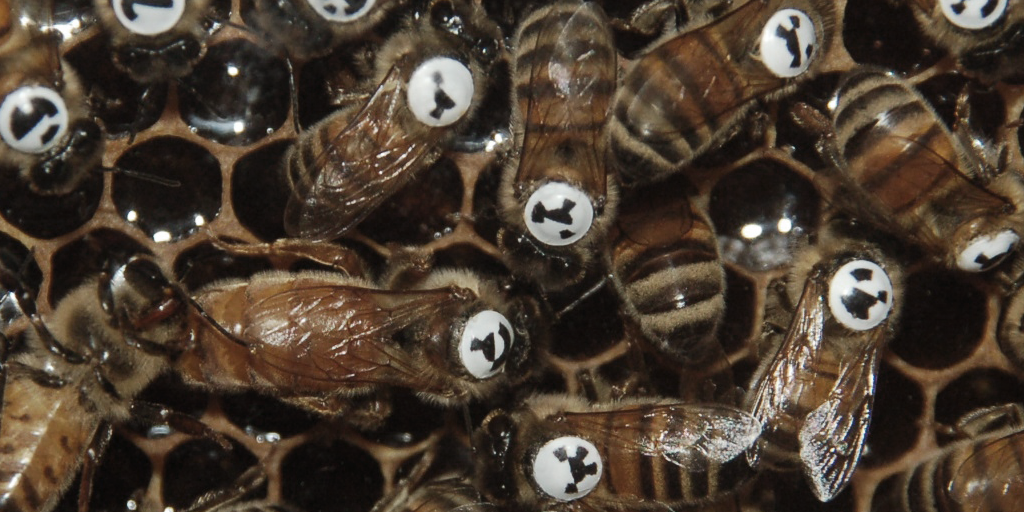
\includegraphics[width=1.0\textwidth]{Figures/markers}
	\caption{Tagged honey bees on the comb. 12-bit cicular tags are used}
	\label{fig:markers}
\end{figure}

\section{Motivation}

Most of the studies analysing behaviour of insects colonies only use a small amount of individually labeled animals, a short observation period, and usually manually detect interaction between animals looking at video data~\cite{quevillon2015social} (hier noch mehr hinmachen TODO).

\section{Research Goal}

Starting off with creating worker-worker interaction networks using spatial proximity as a proxy for interactions between bees.



\section{Methodology}

\section{Outline}